\subsection[平面与直线]{Lines and Planes in $\mathbb{R}^3$}

\subsubsection[平面方程]{Plane}
$2$-dim'l affine subspace.

\begin{itemize}
    \item (General Equation) $\Pi:\,ax+by+cz+d=0$ \allbold{Implicit equation}

          Suppose $r_0=\left(x_0,y_0,z_0\right)\in\Pi$, i.e. $ax_0+by_0+cz_0+d=0$
          \begin{align*}
              ax+by+cz+d=0 & \iff a\left(x-x_0\right)+b\left(y-y_0\right)+c\left(z-z_0\right)=0                                                                                                       \\
                           & \iff \underset{\emph{\text{(Point-Norm Form 点法式)}}}{\left<\overrightarrow{r}-\overrightarrow{r_0},\overrightarrow{n}\right>}=0\text{ where }\overrightarrow{n}=(a,b,c)^T
          \end{align*}
    \item (Point-Directions Form) Take $\underset{\substack{\downarrow\\P}}{\overrightarrow{r_0}}\in\Pi,\,Q,R\in\Pi$, s.t. $\overrightarrow{PQ},\overrightarrow{PR}$ linearly independent, $\overrightarrow{u}=\overrightarrow{PQ},\,\overrightarrow{v}=\overrightarrow{PR}$, then $\Pi$ can be explicitly parameterized by
          $$\overrightarrow{r}=\overrightarrow{r_0}+s\overrightarrow{u}+t\overrightarrow{v}$$
          \emph{$\overrightarrow{n}=\overrightarrow{PQ}\times\overrightarrow{PR}$ normal vector to $\Pi$}
\end{itemize}

\subsubsection[直线方程]{Line}
$1$-dim'l affine subspace, i.e. shift of $1$-dim'l vector subspace.

\begin{itemize}
    \item (Point-Direction Form) $\overrightarrow{r}=\overrightarrow{r_0}+t\overrightarrow{v},\,t\in\mathbb{R}$ \allbold{Explicit equation 显式表达}
    \item (Plane-Intersection) The set of $\mathbb{R}^3$ defined by $\begin{cases}
                  a_1x+b_1y+c_1z+d_1=0 \\
                  a_2x+b_2y+c_2z+d_2=0
              \end{cases}$, satisfying $\text{rk}\begin{pmatrix}
                  a_1 & b_1 & c_1 \\
                  a_2 & b_2 & c_2
              \end{pmatrix}=2$. \allbold{Implicit equation 隐式表达}
\end{itemize}

\emph{\begin{itemize}
        \item (1)$\implies$(2) $\left(\overrightarrow{r}-\overrightarrow{r_0}\right)\times\overrightarrow{v}=\overrightarrow{0}$
              \begin{align*}
                  \begin{pmatrix}
                      i     & j     & k     \\
                      x-x_0 & y-y_0 & z-z_0 \\
                      l     & m     & n
                  \end{pmatrix}=0 & \implies\begin{cases}
                                                n\left(y-y_0\right)=m\left(z-z_0\right) \\
                                                l\left(z-z_0\right)=n\left(x-x_0\right) \\
                                                m\left(x-x_0\right)=l\left(y-y_0\right)
                                            \end{cases} \\
                                           & \implies\left(\begin{array}{ccc|c}
                                                               0  & n & -m & * \\
                                                               -n & 0 & l  & * \\
                                                               m  & l & 0  & *
                                                           \end{array}\right)
              \end{align*}
        \item (2)$\implies$(1) $\overset{\substack{\text{Particular solution}\\\uparrow}}{\overrightarrow{r_0}}+t\left(\overrightarrow{n_1}\times\overrightarrow{n_2}\right)$ where $\overrightarrow{n_1}=\left(a_1,b_1,c_1\right)^T,\overrightarrow{n_2}=\left(a_2,b_2,c_2\right)^T$
    \end{itemize}}

\subsubsection{Relation between Lines \& Planes}

\begin{enumerate}
    \item Two planes: $\begin{cases}
                  \Pi_1:\,a_1x+b_1y+c_1z+d_1=0 & \leadsto \overrightarrow{n_1} \\
                  \Pi_2:\,a_2x+b_2y+c_2z       & \leadsto \overrightarrow{n_2}
              \end{cases}$
          \begin{enumerate}
              \item Parallel: $\overrightarrow{n_1}\parallel \overrightarrow{n_2}$
              \item Intersecting: ``$\theta=\arccos\frac{\left<\overrightarrow{n_1},\overrightarrow{n_2}\right>}{\left|\overrightarrow{n_1}\right|\left|\overrightarrow{n_2}\right|}$''
          \end{enumerate}
    \item Point \& line: $\text{d}(P,L)=\frac{\left|\left(\overrightarrow{r}-\overrightarrow{r_0}\right)\times\overrightarrow{v}\right|}{\left|\overrightarrow{v}\right|}$ 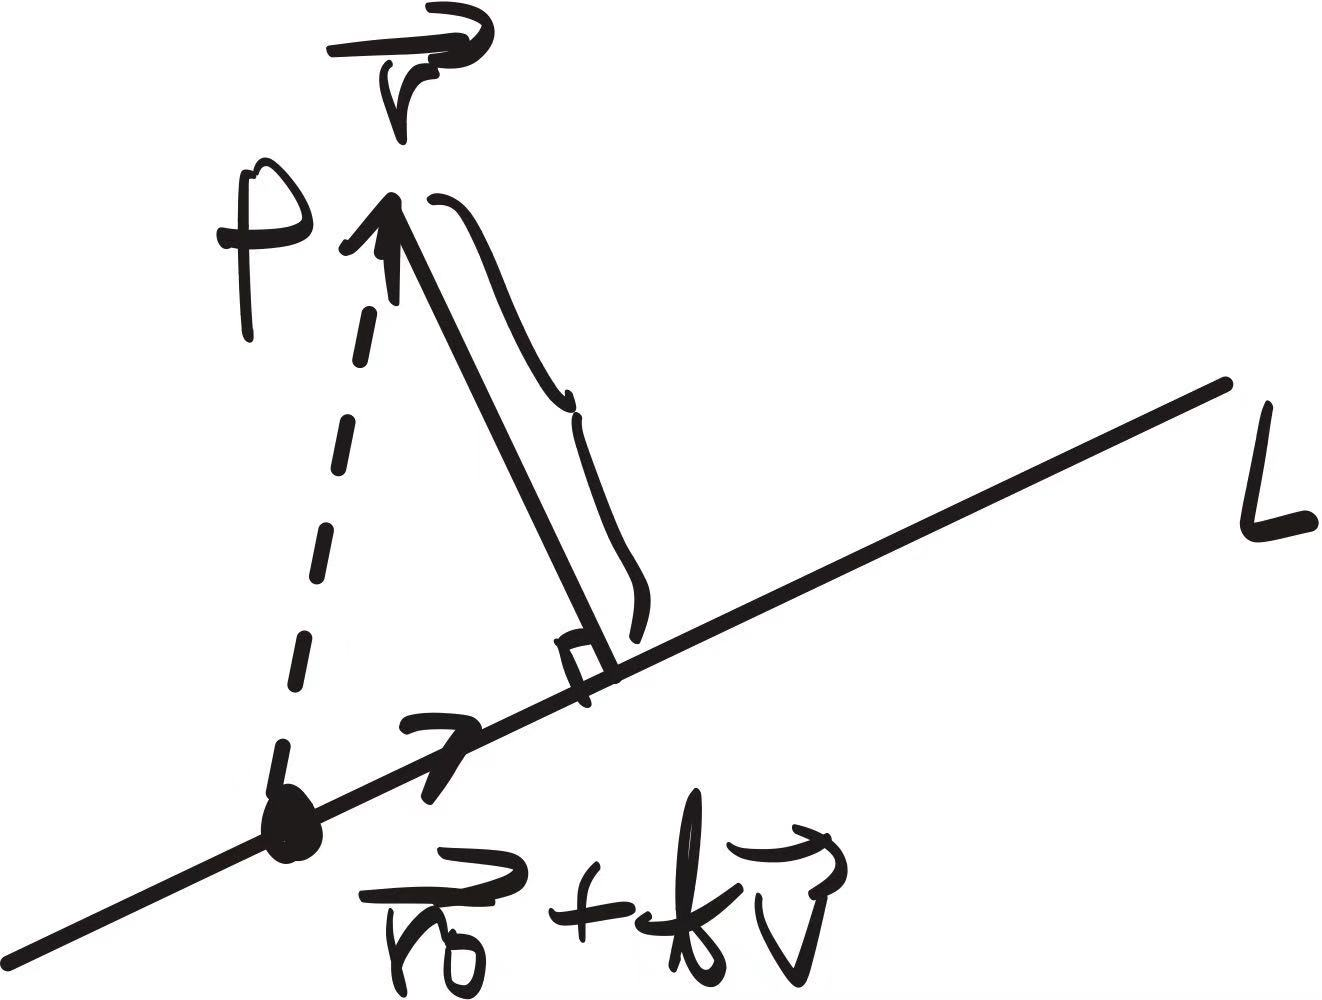
\includegraphics[height=2cm]{chapters/08/PnL}

          Point \& plane: $\underset{P=\begin{pmatrix}
                      x \\
                      y \\
                      z
                  \end{pmatrix}}{\Pi}:\,ax+by+cz+d=0\implies\text{d}(P,\Pi)=\frac{\left|ax+by+cz+d\right|}{\sqrt{a^2+b^2+c^2}}$

          \emph{$\text{d}(P,\Pi)=\left(\overrightarrow{r}-\overrightarrow{r_0}\right)\cdot\overrightarrow{n}=\frac{\left(a\left(x-x_0\right)+b\left(y-y_0\right)+c\left(z-z_0\right)\right)}{\sqrt{a^2+b^2+c^2}}$}
    \item Two lines: $\begin{cases}
                  L_1:\,\overrightarrow{r}=\overrightarrow{r_1}+t\overrightarrow{v_1} \\
                  L_2:\,\overrightarrow{r}=\overrightarrow{r_2}+t\overrightarrow{v_2}
              \end{cases}$
          \begin{enumerate}
              \item Co-planar $\iff\left<\overrightarrow{r_1}-\overrightarrow{r_2},\overrightarrow{v_1}\times\overrightarrow{v_2}\right>=0$
              \item Distance: $\left<\overrightarrow{r_2}-\overrightarrow{r_1},\frac{\overrightarrow{v_1}\times\overrightarrow{v_2}}{\left|\overrightarrow{v_1}\times\overrightarrow{v_2}\right|}\right>$
          \end{enumerate}
\end{enumerate}